\documentclass[conference]{IEEEtran}
\usepackage{graphicx} % Required for inserting images

\title{TP3 Report - Perception and AI}
\author{\IEEEauthorblockN{Bruno Luiz Dias Alves de Castro}
\IEEEauthorblockA{\textit{ESIEE Paris}}
\and
\IEEEauthorblockN{Victor Gabriel Mendes Sündermann}
\IEEEauthorblockA{\textit{ESIEE Paris}}
}
\date{January 2024}

\begin{document}

\maketitle

\section{Introduction}

Autonomous vehicles are one of the most studied and researched topics in Computer Science, Computer Vision and AI. It is a complex problem by nature, and the amount of (literal and figurative) moving parts in this problems attract scientist and developers from all areas.

One of the most important features from an autonomous vehicle, is its ability to recognize people in front of it, and act accordingly. This recognition is no easy task though: the sensors and is locations, the environment, the algorithms and AI behind it, all play critical roles that impact significantly the final result. And being such a sensible feature from such vehicles, a good pedestrian recognition may be what gets a vehicle approved in certain markets, or assure their failure.

Naturally, developing a good network to recognize pedestrians in different scenarios, and using different sensors is extremely important, and that is why we were tasked with such task.

\subsection{Objectives}

The objectives from this practical work are simple and straight forward: develop a network capable of properly recognizing pedestrian in a video footage, using two types of data: a regular video stream, and an infrared footage.

The network developed must be deployed and tested in two circumstances: with and without GPU, and with such evaluate the possibility of deploying out network in a real world scenario.

\section{Data preparation}

The first step in our development, was preparing the data we had for training and validation. For this, we were provided with frames from real video footage captured in a car. Our task was to select a few of these frames that contain pedestrians in them, and highlight them, using a rectangle. There are multiple ways this task could have been done, but we chose a software called \textit{\textbf{Roboflow}}.

\subsection{Roboflow}

\textit{\textbf{Roboflow}} is a web framework focused on data preparation and dataset development. It provides us with all the tools needed for classifying and prepossess our images. It also provides us easy methods of deployment, such as an API, to better import our datasets into our projects without the need to juggle files around.

The dataset prepared with \textit{\textbf{Robolow}} was imported into a \textit{\textbf{Python Notebook}}, and the project development followed, using \textit{\textbf{Google Colab}}.

\section{Development}

Among all the technologies used during this project, a few can be highlighted:

\begin{itemize}
    \item \textit{\textbf{Ultralytics}}: a library that helps us retrieving data such as performance and specifications from our CPU.
    \item \textit{\textbf{YOLO}}: a real-time object detection system from \textit{\textbf{Ultralytics}}, trained in our project.
    \item \textit{\textbf{OpenCV}}: a optimized Computer Vision library that provides tools and hardware.
\end{itemize}

We decided to use YOLO as the detection network because it is a state of the art system, being both fast and accurate when compared to other famous systems, like RetinaNet or SSD.

An essential part in this work is data preparation, in order for the network to be as effective as possible we created a database comprised of 168 annotated images. We applied various augmentation methods in the images to further train our network, resulting in a total of 436 images divided as 92\% training and 8\% validation.

The training of our network was done in 25 epochs and using two different hardware. First we ran the program on the CPU, and later we focused on the use of the GPU. The learning rates and the detection results are laid out in the following subsections.

\subsection{CPU Implementation}
The CPU execution unfortunately didn't bring any satisfactory results, likely because the network was trained in such a small number of epochs, and most likely didn't get to learn how to detect people. It is also important to note that the training took 18.7 minutes, and that the analysis of a single frame of the video took 33 ms on average. Figures 1, 2 and 3 show the metrics achieved by our network after training.

\begin{figure}[ht!]
    \centering
    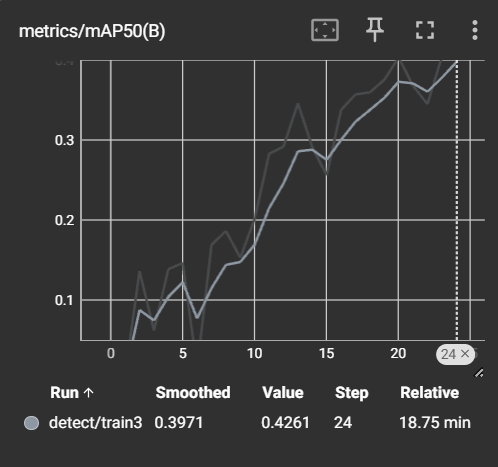
\includegraphics[width=0.4\textwidth]{Images/CPU/Screenshot 2024-01-27 185829.png}
    \caption{Mean Average Precision for CPU}\label{fig:CPUmAP}
\end{figure}

\begin{figure}[ht!]
    \centering
    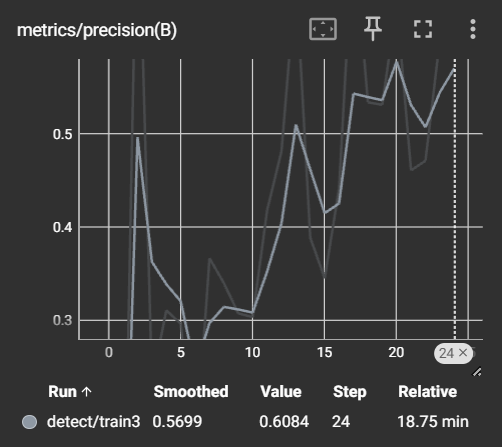
\includegraphics[width=0.4\textwidth]{Images/CPU/Screenshot 2024-01-27 185928.png}
    \caption{Precision for CPU}\label{fig:CPUprecision}
\end{figure}

\begin{figure}[ht!]
    \centering
    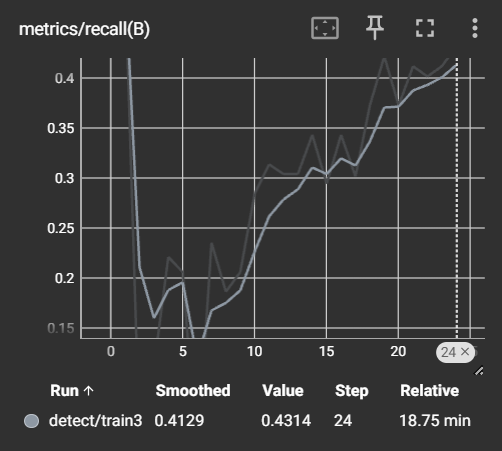
\includegraphics[width=0.4\textwidth]{Images/CPU/Screenshot 2024-01-27 185951.png}
    \caption{Recall for CPU}\label{fig:CPUrecall}
\end{figure}

\subsection{GPU Implementation}
The metrics of this test were slightly better than the ones generated by the CPU, on top of that we can see that the execution time for training the network was drastically reduced, taking approximately 2.6 minutes. Figures 4, 5 and 6 show the metrics obtained by our network after training.
\begin{figure}[ht!]
    \centering
    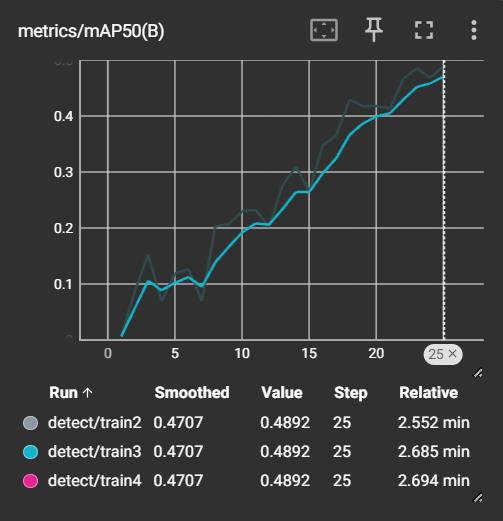
\includegraphics[width=0.35\textwidth]{Images/GPU/Screenshot 2024-01-27 182452.png}
    \caption{Mean Average Precision for GPU}\label{fig:GPUmAP}
\end{figure}

\begin{figure}[ht!]
    \centering
    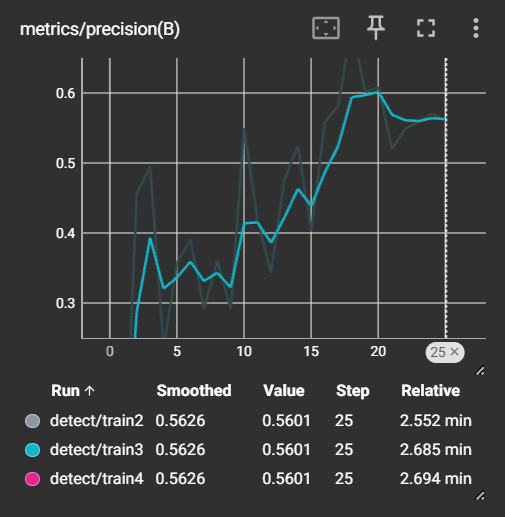
\includegraphics[width=0.35\textwidth]{Images/GPU/Screenshot 2024-01-27 182658.png}
    \caption{Precision for GPU}\label{fig:GPUprecision}
\end{figure}

\begin{figure}[ht!]
    \centering
    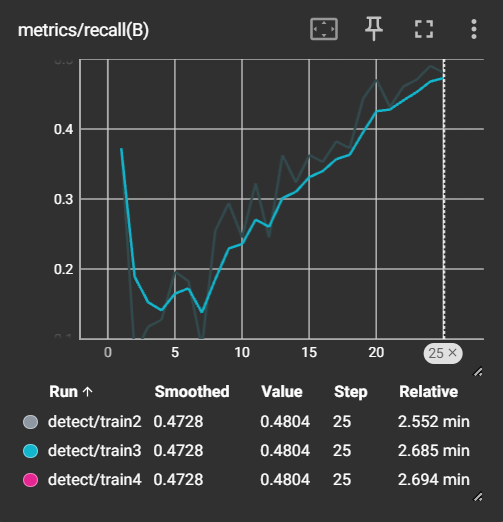
\includegraphics[width=0.35\textwidth]{Images/GPU/Screenshot 2024-01-27 182608.png}
    \caption{Recall for GPU}\label{fig:GPUrecall}
\end{figure}

\subsubsection{Results}
When predicting the video, we got underwhelming results, shown in pictures 7, 8 and 9. Our model detects only a few people, even thought there is a crowd passing. We can also observe that the confidence of the model isn't very high, resulting from the small number of epoch during training. However the analysis of each frame takes only 15 ms, less than half of the time of the CPU.

\begin{figure}[ht!]
    \centering
    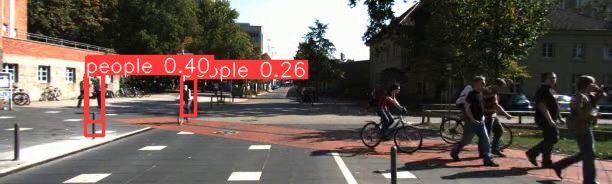
\includegraphics[width=0.4\textwidth]{Images/GPU/download (2).png}
    \caption{Network result 1}\label{NetRes1}
\end{figure}

\begin{figure}[ht!]
    \centering
    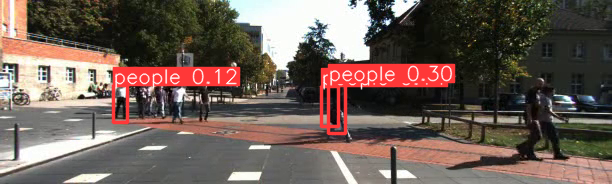
\includegraphics[width=0.4\textwidth]{Images/GPU/download (4).png}
    \caption{Network result 2}\label{fig:NetRes2}
\end{figure}

\begin{figure}[ht!]
    \centering
    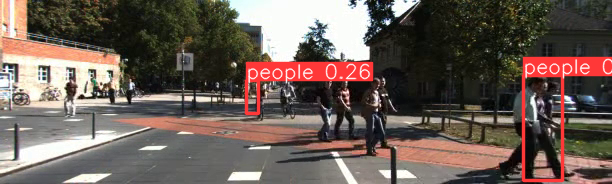
\includegraphics[width=0.4\textwidth]{Images/GPU/download (3).png}
    \caption{Network result 3}\label{fig:NetRes3}
\end{figure}

\subsection{Infrared Training}
Alongside the regular dataset, with standard RGB video recordings, we also classified and preprocessed a similar dataset with Infrared (IR) video footage. For this implementation, knowing the CPU takes a long time to run, and performs worse, we decided to only train it on the GPU.

\subsubsection{Results}
The results obtained with with this dataset were (at least with the dataset we had) significantly better. The model was able to detect more people in the images, and had less false positives.

\begin{figure}[ht!]
    \centering
    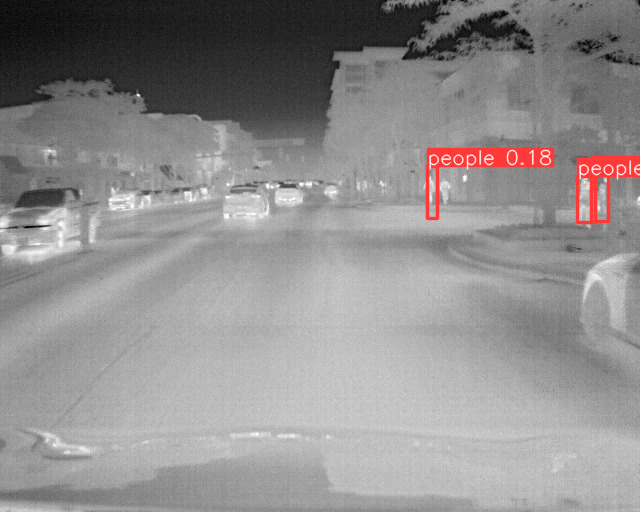
\includegraphics[width=0.4\textwidth]{Images/ir_result.png}
    \caption{IR Results}\label{fig:ir-results}
\end{figure}

\section{Conclusion}
Object recognition is a difficult task. The variables involved are complex to balance, and any small thing may have a huge impact in the end result. Especially in a field such as autonomous vehicles, where time and precision are crucial, this problem proves to be way harder than we first thought.

In all our implementations, we were not able to reach acceptable accuracy levels, and the timing is less than optimal for such a task, especially in the CPU training implementation. A form of graphics/AI acceleration proves indispensable for this task.

Our models, though far from perfect, do serve as an exciting first contact with this field. The results we got are promising, however we are sure that with more time, data and resources available, we could reach better numbers.

\end{document}
